\clearpage
\begin{flushright}
	\textit{Лекция №5}
	\textit{2015.09.22}
\end{flushright}

Переключение полного контекста – долго. Аппаратного – поддерживается на аппаратном уровне.
???
Устройству выделяются и другие ресурсы. Семафоры, ???. Вся эта информация составляет полный контекст. Она фиксируется в структурах. На них ссылается основная структура, описывающая процесс. В Unix это struct proc. Стараясь сократить временные расходы в прошлом веке была введена концепция потоков. Поток – непрерывная часть кода, грубо говоря: кусок кода, такие части кода могут выполняться параллельно. Чтобы они могли выполняться параллельно их оформляют в виде потоков. 
В Windows – каждый запущенный драйвер – это поток. 

\paragraph{Виды потоков}: 
\begin{enumerate}
    \item Потоки ядра;
    \item Легковесные процессы. Потоки уровня ядра. Владельцем ресурсов является процесс, а потоку принадлежит счетчик команд и аппаратный контекст. При этом надо сказать, что выигрыш если переключаемся между потоками одного процесса, но если к потоку другого процесса, то происходит переключение полного контекста;
    \item Пользовательские нити. Для управления необходима специальная библиотека потоков. Должна предоставлять функции планирования потоков, диспетчеризации, сохранения контекста. Как только поток запросил функции ядра, то процесс приостанавливается, пока не завершиться операция ядра (например: ввода – вывода).
\end{enumerate}

Поток выполняется в адресном пространстве процесса. Таблицы, описывающие память, принадлежат процессу. Адресное пространство процесса описывается соответствующими таблицами. Для взаимодействия потоков можно использовать глобальные переменные. Процессы имеют защищенные адресные пространства, в том смысле что ни один процесс не может обратиться за собственное адресное пространства.

\begin{table}[H]
\caption{Однопоточная модель процесса.}
\begin{tabular}{|l|}
\hline
Блок управления процессом\\
\hline
Стек ядра\\
\hline
Стек пользователя\\
\hline
Адресное пространство пользователя\\
\hline
\end{tabular}
\end{table}

\begin{figure}[H]
	\centering
	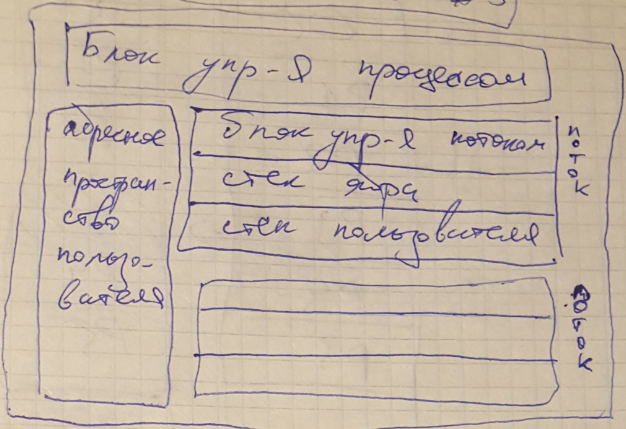
\includegraphics[width=\textwidth]{pic/1.png}
	\caption{Многопоточная модель процесса}
\end{figure}

Поток представляется системе дескриптором (блок управления потоком). У каждого потока есть стека ядра. Чтобы сохранять контекст (системный контекст) используется стек ядра. Нельзя использовать стек пользователя, потому что пользователь может создать несколько стеков, назначать им размеры. \cite{Kuznets_blesk}

\chapter{Процессы ОС Unix}

\section{Системный вызов fork()}. Создает новый процесс. В Unix все процессы создаются единообразно вызовом \verb|fork()|. Любой процесс может создать любое кол-во процессов. При этом процессы в Unix находятся в отношении предок – потомок. В результате создается иерархия процессов.  \verb|fork()| является базовым примитивом. 
В ANCI C не хорошо писать большими буквами, так как много предопределенных констант написаны с больших букв. 

\begin{figure}[H]
	\centering
	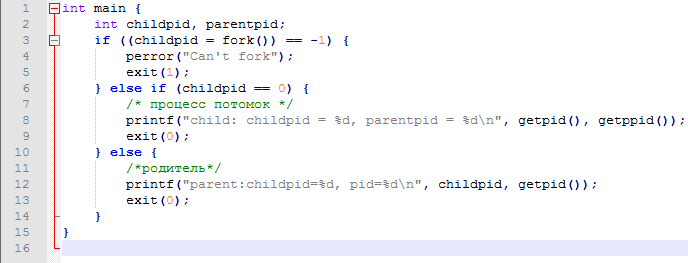
\includegraphics[width=\textwidth]{pic/2.png}
	\caption{listing}
	\label{listing:fork}
\end{figure}

В результате \verb|fork()| создается копия процесса предка, в том смысле, что процесс-потомок на следует код предка, дескрипторы открытых файлов, сигнальную маску.

Замечание 1. В Unix всё файл, внешние устройства тоже файлов.

В старых системах Unix (для pdp 11) код предка копировался в адресное пространство потомка. В результате в системе могло существовать одновременно большое количество копий одной и той же программы.  Память используется неэффективно. В современных системах используется умный fork, который реализуется следующим образом: для процесса – потомка создаются собственные карты трансляции адресов (таблица страниц), которые ссылаются на страницы адресного пространства предка, т.е. в таблицы страниц потомка находятся дескрипторы страниц адресного пространства предка (адреса страниц адресного пространства предка). Pointer – указатель (не типизированный). Reference – ссылка (типизированный). Процесс-потомок получается собственные карты трансляции адресов, и эти таблицы страниц ссылаются на страницы адресного пространства предка. Но процессы имеют особенность обращаться к собственные страницы, и писать в свои страницы сегменты данных или стека. Процесс не заинтересован в тех изменения другого процесса. Решено штукой copy on write. Для страниц предка (сегмента данных и стека) меняется права доступа на «только для чтения» и устанавливается флаг copy on write. Флаг copy on write. Если или предок, или потомок пытаются изменить страницу, то возникнет исключение по правам доступа. Обрабатывая это исключение, супервизор (ОС в стадии выполнения) обнаружит установленный флаг copy on write и создаст копию страницы в адресном пространстве того процесса, который пытался её изменить. В результате в системе создается необходимое количество копий (отдельных страниц). Это будет действовать до тех пор, пока процесс потомок не вызовет или системный вызов \verb|exec()| или системный вызов \verb|exit()|. Если потомок сделал эти системные вызовы, то страницы предка получают обычные права (read / write) и флаг copy on write сбрасывается. 

\section{Системный вызов exec()}.
В Unix предлагается системный вызов exec(), который переводит процесс на новое адресное пространство программы, которая указана в системном вызове \verb|exec(), execl(), execv(), execle(“/bin/ls”, “ls”, “-l”, 0);|, где
$/bin/ls$ - исполняемая программа, которая выводит на экран список файлов

Системный вызов \verb|exec()| создает низкоуровневый процесс.  Не создают полноценный процесс, но выполняют действие, которое связано с созданием нового процесса. Создание нового адресного пространства. Системный вызов \verb|exec()| создает карты трансляции адресов для адресного пространства программы, которая передана в системному вызову \verb|exec()| в качестве параметра.  \verb|exec()| создает новые таблицы страниц, которая ссылается на новую программу в параметрах \verb|exec()|. После этого \verb|exec()| заменяет адресное пространство потомка на вновь созданное адресного пространств. Идет замена одной таблицы на другую выполняется простой замены адреса. В Intel есть регистр $CR3$ , который содержит начальный адрес таблиц страниц. При переключении процессов заменяются адреса в регистрах процессора. \verb|exec()| создает новое адресное пространство, это значит его описать, создать для этого адресного пространства соответствующие таблицы. Переход на новое адресное пространство осуществляется простой заменой адреса. Мы теряем указатель на эту таблицу и она превращается в мусор. 

\section{Иерархия процессов.}

\begin{figure}[H]
	\centering
	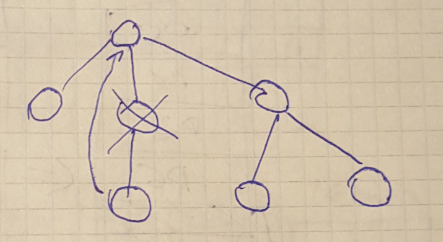
\includegraphics[width=\textwidth]{pic/3.png}
	\caption{Иерархия процессов}
\end{figure}

В результате \verb|fork()| предок получает id созданных потомков. Смотрим в \verb|struct proc|, там есть указатель на самого последнего созданного потомка. Потомков может быть создано любое кол-во, поэтому это – связный список. В результате \verb|fork()| создается иерархия процессов, которые связанны отношением предок – потомок. Процесс предок может завершиться раньше потомка, если не предпринять специальных действий, то иерархия процессов разрушиться. Процесс, у которого завершился предок, называется \textbf{сиротой}. Система предпринимает ряд действий для сохранения иерархии процессов. 

Unix поддерживает понятие терминал программно. И Unix и Windows являются системами (реального ???) времени, это когда к компу подключены терминалы. Мы можем запустить любое количество терминалов. В Windows это консоль. 
Когда запускаем систему, то запускается процесс init с id = 0. Когда открываем терминал, то создается процесс ???. Терминальный процесс (id = 1) является предком всех процессов, запущенных в данном терминале. 

Код в \ref{listing:fork} чреват тем, что предок может завершиться раньше потомков.  При завершении любого процесса система проверяет, не остались ли у него незавершенные потомки, если такие процессы – потомки у него остались, то выполняются действия по усыновлению осиротевших процессов терминальным процессом. Для этого модифицируются соответствующие дескрипторы. Процесс потомок в parrantid получает id терминального процесса, а терминальный процесс получает указатель на осиротевший процесс. При завершении потомков процессы-предки получают статусы завершения своих потомков. Если произошло усыновление, то статус завершения получит терминальный процесс. 